% -*- TeX:de -*-
\NeedsTeXFormat{LaTeX2e}
\documentclass[12pt,a4paper]{article}
\usepackage[english]{babel} % german text
\usepackage[DIV12]{typearea} % size of printable area
\usepackage[T1]{fontenc} % font encoding
%\usepackage[latin1]{inputenc} % most likely on Windows
\usepackage[utf8]{inputenc} % probably on Linux
\usepackage{multicol}
% PLOTTING
\usepackage{pgfplots}
\usepackage{pgfplotstable}
\usepackage{url}
\usepackage{graphicx} % to include images
\usepackage{tikz}
\usepackage{subfigure} % for creating subfigures
\usepackage{amsmath} % a bunch of symbols
\usepackage{amssymb} % even more symbols
\usepackage{booktabs} % pretty tables
\usepackage{makecell} % multi row table heading
% a floating environment for circuits
\usepackage{float}
\usepackage{caption}
\usepackage{hyperref}

% Title Page command
\newcommand{\HRule}{\rule{\linewidth}{0.5mm}}

%\newfloat{circuit}{tbph}{circuits}
%\floatname{circuit}{Schaltplan}
% a floating environment for diagrams
%\newfloat{diagram}{tbph}{diagrams}
%\floatname{diagram}{Diagramm}
\pgfplotsset{compat=1.8}
\selectlanguage{english} % use german
\begin{document}
%%%%%%% DECKBLATT %%%%%%%
\begin{titlepage}
\begin{center}

% Upper part of the page. The '~' is needed because \\
% only works if a paragraph has started.

\includegraphics[scale=0.75]{./unilogo}~\\[2cm]

\textsc{\LARGE University of Vienna }\\[0.5cm]
\textsc{\LARGE Faculty of Physics}\\[1.5cm]
\textsc{\Large Quantum optics practical course}\\[0.5cm]

% Title
\HRule \\[0.4cm]
{ \huge \bfseries Radiaton Pressure}\\[0.4cm]

\HRule \\[1.5cm]

% Author and supervisor
\begin{minipage}{0.4\textwidth}
\begin{flushleft} \large
\emph{Author:}\\
Johannes \textsc{Kurz}\\
\emph{Group:}\\
\textsc{Braun, Donabaum, Kurz}\\
\end{flushleft}
\end{minipage}
\begin{minipage}{0.4\textwidth}
\begin{flushright} \large
\emph{Supervisor:} \\
Witlef \textsc{Wieczorek}
\end{flushright}
\end{minipage}

\vfill

% Bottom of the page
{\large 31.10.2014}

\end{center}
\end{titlepage}
%%%%%%% DECKBLATT ENDE %%%%%%%
\pagebreak
\setlength{\columnsep}{20pt}
\begin{multicols}{2}

\begin{abstract}

\end{abstract}

%%%%%%%%%%%%%%%%%%%%%%%%%%%%%%%%%%%%%%%%%%%%%%%%
%\begin{figure}[H]
% \centering
% \includegraphics[scale=0.35]{./data/beugung.png}
% \caption{Beugungsmuster Einzelspalt (echtes Foto; schwarz durch weiß ersetzt)}
% \label{fig:beugungsmuster}
%\end{figure}
%\begin{figure}[H]
% \centering
% \pgfplotstabletypeset[
% columns={abstand, n},
% col sep=&,
% columns/abstand/.style={precision=2, zerofill, column name=\makecell{$Abstand$\\$(\pm 0.05)[mm]$} },
% columns/n/.style={column name=\makecell{$n$\\$(Ordnung)$}, precision=0},
% every head row/.style={before row=\hline,after row=\hline\hline},
% every last row/.style={after row=\hline},
% every first column/.style={column type/.add={|}{} },
% every last column/.style={column type/.add={}{|} }
% ]{
% abstand & n
% 12.9 & 1
% 24.45 & 2
% 37.40 & 3
% 49.35& 4
% 62.45 & 5
% 74.45 & 6
% 87.45 & 7
% 100.25 & 8
%
% }
% \caption{Messwerte Einzelspalt}
% \label{tab:werte_einzelspalt}
%\end{figure}
%%%%%%%%%%%%%%%%%%%%%%%%%%%%%%%%%%%%%%%%%%%%%%%%
%%%%%%%%%%%%%%%%%%%%%%%%%%%%%%%%%%%%%%%%%%%%%%%%

\section{Radiation pressure}
Goal of this work is to demonstrate how massless photons counter intuitively create pressure based on quantum mechanical
properties.
On the following pages the theoretical basics will be explained and enhanced to fit the experiment.
The Experiment itself will be explained in further sections. Results and discussion about the outcome
will complete this work.

%%%%%%%%%%%%%%%%%%%%%%%%%%%%%%%%%%%%%%%%%%%%%%%%
%%%%%%%%%%%%%%%%%%%%%%%%%%%%%%%%%%%%%%%%%%%%%%%%
\section{Theory}
The foundation of photons inducing a pressure comes from the photoelectric effect where (Max Planck) stated that:
$$E = h * \nu$$
The energy E of a photon is proportional to the Planck constant times the frequency $\nu$.
From this knowledge combined with (Einstein's) law $E = m * c^2$ we can derive a mass:
$$m = \frac{h * \nu}{c^2}$$
Combined with the classical definition of momentum $p = m * v$ we get:
$$p = \frac{h * \nu}{c^2} * c = \frac{h * \nu}{c}$$
Due to the fact that pressure is defined as force per square meter we can get the pressure by the time derivative of the momentum times the number of particles per area element.

\subsection{Cantilever}
A cantilever is a high (> 99\%) reflective mirror with the diameter of about a millimeter. The size may vary concerning the usage. In example a photon trap may have bigger mirrors (also convex etc).\\ 
The mirror in our case is mounted on a long rod so it can oscillate back and forth.
High reflectivity is needed because the highest force transfer and therefore pressure is obtained when all photons are reflected.

\subsection{Dampend driven harmonic oszilliation}
With a pulsed laser and a previous described cantilever we can build a oscillator that responds to the force of the photons. Because we want to measure a very tiny pressure the cantilever has to be driven by the pulsed laser at the resonance frequency of the oscillator. Due to the fact that we don't cool or evacuate our setup we have a dampening that is overcome by the repeated pulsing of the laser with the resonance frequency.\\
The calculation of the oscillator is stated in the experimental description \cite{physikwiki}.

%%%%%%%%%%%%%%%%%%%%%%%%%%%%%%%%%%%%%%%%%%%%%%%%
%%%%%%%%%%%%%%%%%%%%%%%%%%%%%%%%%%%%%%%%%%%%%%%%
\section{Experimental assembly}
We have a build up table top experiment composed of different components.

%%%%%%%%%%%%%%%%%%%%%%%%%%%%%%%%%%%%%%%%%%%%%%%%
%%%%%%%%%%%%%%%%%%%%%%%%%%%%%%%%%%%%%%%%%%%%%%%%
\section{Results}
\cite{github}

\begin{figure}[H]
	\centering
	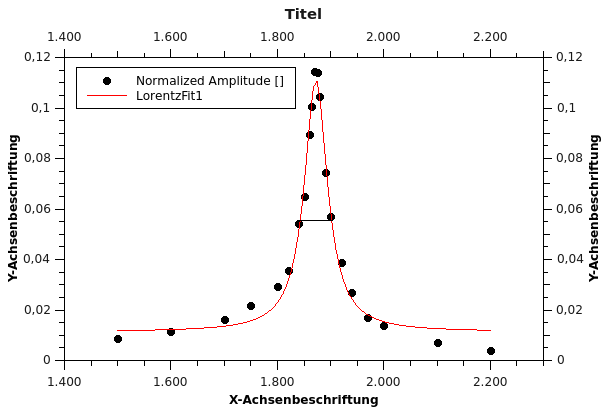
\includegraphics[scale=1.2]{../figures/Resonanzkurve.png}
	\caption{Resonanzkurve}
	\label{fig:resonanzkurve}
\end{figure}
%%%%%%%%%%%%%%%%%%%%%%%%%%%%%%%%%%%%%%%%%%%%%%%%
%%%%%%%%%%%%%%%%%%%%%%%%%%%%%%%%%%%%%%%%%%%%%%%%
\section{Discussion}
tba

%%%%%%%%%%%%%%%%%%%%%%%%%%%%%%%%%%%%%%%%%%%%%%%%
%%%%%%%%%%%%%%%%%%%%%%%%%%%%%%%%%%%%%%%%%%%%%%%%
\pagebreak

\bibliography{protocol.bib}
\bibliographystyle{plain}

\end{multicols}
\end{document}